\subsection{Recalculating micro-spreadsheet using Z3Py}

There is a nice exercise\footnote{Blog post in Russian: \url{http://thesz.livejournal.com/280784.html}}:
write a program to recalculate micro-spreadsheet, like this one:

\lstinputlisting{SMT/spreadsheet/test1}

As it turns out, though overkill, this can be solved using Z3 with little effort:

\lstinputlisting{SMT/spreadsheet/1.py}

( \url{https://github.com/DennisYurichev/yurichev.com/blob/master/blog/spreadsheet/1.py} )

All we do is just creating pack of variables for each cell, named A0, B1, etc, of integer type.
All of them are stored in \textit{cells[]} dictionary.
Key is a string.
Then we parse all the strings from cells, and add to list of constraints \textit{A0=123}
(in case of number in cell) or \textit{A0=B1+C2} (in case of expression in cell).
There is a slight preparation: string like \textit{A0+B2} becomes \textit{cells["A0"]+cells["B2"]}.

Then the string is evaluated using Python \textit{eval()} method,
which is highly dangerous
\footnote{\url{http://stackoverflow.com/questions/1832940/is-using-eval-in-python-a-bad-practice}}:
imagine if end-user could add a string to cell other than expression?
Nevertheless, it serves our purposes well, because this is a simplest way to pass a string with expression into Z3.

Z3 do the job with little effort:

\begin{lstlisting}
 % python 1.py test1
sat
1       0       135     82041
123     10      12      11
667     11      1342    83383
\end{lstlisting}

\subsubsection{Unsat core}

Now the problem: what if there is circular dependency? Like:

\lstinputlisting{SMT/spreadsheet/test_circular}

Two first cells of the last row (C0 and C1) are linked to each other.
Our program will just tells ``unsat'', meaning, it couldn't satisfy all constraints together.
We can't use this as error message reported to end-user, because it's highly unfriendly.

However, we can fetch \textit{unsat core}, i.e., list of variables which Z3 finds conflicting.

\begin{lstlisting}
...
s=Solver()
s.set(unsat_core=True)
...
        # add constraint:
        s.assert_and_track(e, coord_to_name(cur_R, cur_C))
...
if result=="sat":
...
else:
    print s.unsat_core()
\end{lstlisting}

( \url{https://github.com/DennisYurichev/yurichev.com/blob/master/blog/spreadsheet/2.py} )

We should explicitly turn on unsat core support and use \textit{assert\_and\_track()} instead of \textit{add()} method,
because this feature slows down the whole process, and is turned off by default.
That works:

\begin{lstlisting}
 % python 2.py test_circular
unsat
[C0, C1]
\end{lstlisting}

Perhaps, these variables could be removed from the 2D array, marked as \textit{unresolved}
and the whole spreadsheet could be recalculated again.

\subsubsection{Stress test}

How to generate large random spreadsheet?
What we can do.
First, create random \ac{DAG}, like this one:

\begin{figure}[H]
\centering
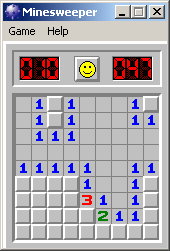
\includegraphics[width=\textwidth]{SMT/spreadsheet/1.png}
\caption{Random DAG}
\end{figure}

Arrows will represent information flow.
So a vertex (node) which has no incoming arrows to it (indegree=0), can be set to a random number.
Then we use topological sort to find dependencies between vertices.
Then we assign spreadsheet cell names to each vertex.
Then we generate random expression with random operations/numbers/cells to each cell,
with the use of information from topological sorted graph.

Wolfram Mathematica:

\begin{lstlisting}
(* Utility functions *)
In[1]:= findSublistBeforeElementByValue[lst_,element_]:=lst[[ 1;;Position[lst, element][[1]][[1]]-1]]

(* Input in 1..∞ range. 1->A0, 2->A1, etc *)
In[2]:= vertexToName[x_,width_]:=StringJoin[FromCharacterCode[ToCharacterCode["A"][[1]]+Floor[(x-1)/width]],ToString[Mod[(x-1),width]]]

In[3]:= randomNumberAsString[]:=ToString[RandomInteger[{1,1000}]]

In[4]:= interleaveListWithRandomNumbersAsStrings[lst_]:=Riffle[lst,Table[randomNumberAsString[],Length[lst]-1]]

(* We omit division operation because micro-spreadsheet evaluator can't handle division by zero *)
In[5]:= interleaveListWithRandomOperationsAsStrings[lst_]:=Riffle[lst,Table[RandomChoice[{"+","-","*"}],Length[lst]-1]]

In[6]:= randomNonNumberExpression[g_,vertex_]:=StringJoin[interleaveListWithRandomOperationsAsStrings[interleaveListWithRandomNumbersAsStrings[Map[vertexToName[#,WIDTH]&,pickRandomNonDependentVertices[g,vertex]]]]]

In[7]:= pickRandomNonDependentVertices[g_,vertex_]:=DeleteDuplicates[RandomChoice[findSublistBeforeElementByValue[TopologicalSort[g],vertex],RandomInteger[{1,5}]]]

In[8]:= assignNumberOrExpr[g_,vertex_]:=If[VertexInDegree[g,vertex]==0,randomNumberAsString[],randomNonNumberExpression[g,vertex]]

(* Main part *) 
(* Create random graph *)
In[21]:= WIDTH=7;HEIGHT=8;TOTAL=WIDTH*HEIGHT
Out[21]= 56

In[24]:= g=DirectedGraph[RandomGraph[BernoulliGraphDistribution[TOTAL,0.05]],"Acyclic"];

...

(* Generate random expressions and numbers *)
In[26]:= expressions=Map[assignNumberOrExpr[g,#]&,VertexList[g]];

(* Make 2D table of it *)
In[27]:= t=Partition[expressions,WIDTH];

(* Export as tab-separated values *)
In[28]:= Export["/home/dennis/1.txt",t,"TSV"]
Out[28]= /home/dennis/1.txt

In[29]:= Grid[t,Frame->All,Alignment->Left]
\end{lstlisting}

Here is an output from \textit{Grid[]}:

\begin{center}
\begin{tabular}{ | l | l | l | l | l | l | l |}
\hline
846 & 499 & A3*913-H4 & ... & ... & ... & ... \\
\hline
B4*860+D2 & 999 & 59 & ... & ... & ... & ... \\
\hline
G6*379-C3-436-C4-289+H6 & 972 & 804 & ... & ... & ... & ... \\
\hline
F2 & E0 & B6-731-D3+791+B4*92+C1 & ... & ... & ... & ... \\
\hline
519 & G1*402+D1*107*G3-458*A1 & D3 & ... & ... & ... & ... \\
\hline
F5-531+B5-222*E4 & 9 & B5+106*B6+600-B1 & ... & ... & ... & ... \\
\hline
C3-956*A5 & G4*408-D3*290*B6-899*G5+400+F1 & B2-701+H6 & ... & ... & ... & .. \\
\hline
B4-792*H4*407+F6-425-E1 & D2 & D3 & ... & ... & ... & ... \\
\hline
\end{tabular}
\end{center}



Using this script, I can generate random spreadsheet of $26 \cdot 500=13000$ cells,
which seems to be processed in couple of seconds.

\subsubsection{The files}

The files, including Mathematica notebook: \url{https://github.com/DennisYurichev/yurichev.com/tree/master/blog/spreadsheet}.

